\documentclass[10pt]{armath}
\usepackage{amsmath}
\usepackage{csquotes}
\usepackage{enumitem}
\usepackage{tikz}

\usepackage[T1]{fontenc}
\usepackage[utf8]{inputenc}
\usepackage{lmodern}

\usepackage[english]{babel}
\usepackage{csquotes}

\usepackage[notes,backend=biber]{biblatex-chicago}
\bibliography{ref.bib}

\title{Ancient Sculpture Polychromy}
\author{Arden Rasmussen}
\date{\today}

\begin{document}
\maketitle

Most sculptures that we have from ancient Greece lack any sign of colors or
pigments. Because of this fact, the casual observer may not even consider that
this was not the intended state. However, through scientific research, analysis
of the sculptures, and cross-referencing with literary material, we know that
this is not the case.  Practically all sculpture and architecture in ancient
Greece was brightly colored. We examine some of the scientific methods that are
utilized to gain insight into the original coloring of a sculpture. This is
becoming very useful in cases where most of the pigments have faded away due to
exposure to light.

The first evidence that ancient sculpture had coloring of any form comes from
the sculptures that were covered in ash in Pompeii. The ash was able to protect
the pigments from the harmful effects of sunlight. Because of this, the
pigments of these sculptures were preserved significantly better than any of
those on previously discovered sculptures. This makes it clear that the
sunlight is a significantly harmful factor when it comes to pigment
preservation.

Many of the early attempts at the inference of the colorization of sculpture
and architecture was done before the discovery of many of the scientific
techniques that are now used today. This means that most reconstructions were
primarily based on the aesthetical preferences of the historian attempting the
restoration. These reconstructions only accounted for a few bits of evidence
that were available at the time. The primary evidence was if the color was
clearly visible on the sculpture; if it was not, then it was up to the
historian to decide what color should be placed there.

As more scientific methods of determining the colorization or the pigment of
sculptures were developed, the accuracy of the reconstructions began to
converge to the ground truth of how they may have been originally painted. We
will go through all of the methods that are now used commonly in order to
assist in the determination of the color or the pigments utilized for ancient
sculpture.

\textbf{Visual Analysis} This is a very simplistic method of analysis for the
determination of colors present on a sculpture. It simply involves visually
looking at different portions of the sculpture. This can either be done by eye
or by using tools for optical enhancement, such as a microscope. By looking at
what remains of sculpture, and depending on how well the sculpture was
preserved, it can be possible to visually identify colors.

\begin{figure}[htpb]
  \centering
  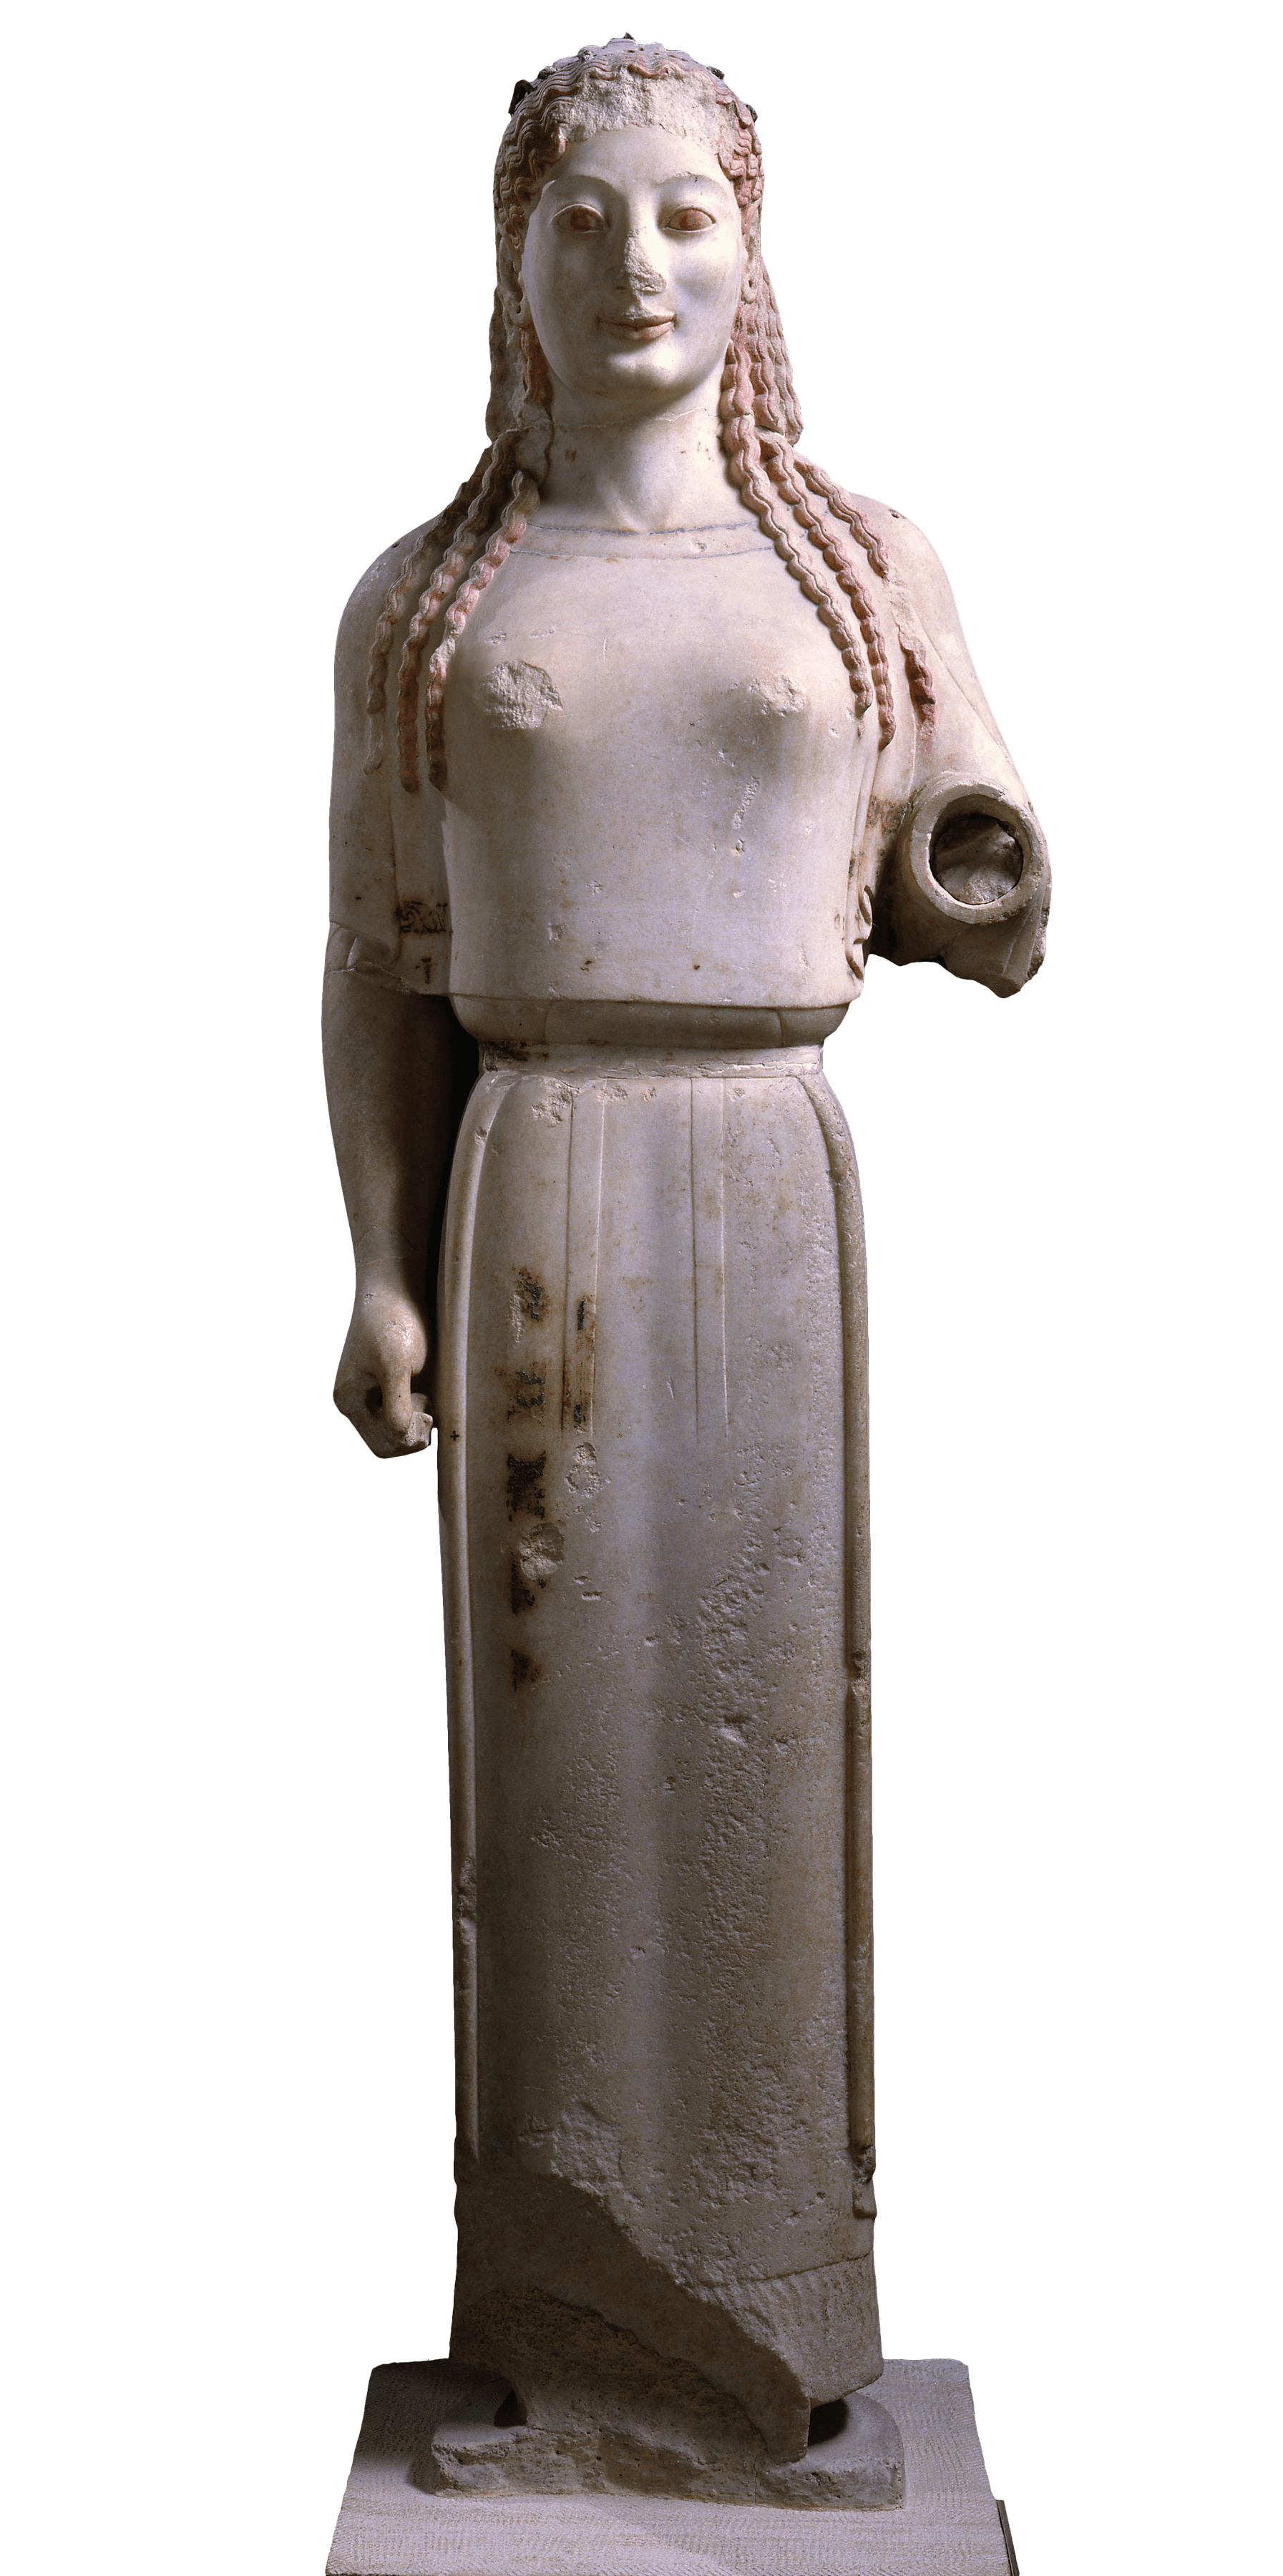
\includegraphics[width=0.4\linewidth]{visual_analysis.png}
  \caption{Peplos Kore, displaying the ability to use visual analysis on
  ancient Greek sculpture.}
  \label{fig:visual_analysis}
\end{figure}

We will describe this process of visual analysis using the example of the
Peplos Kore from the Acropolis (539BCE) shown in figure
\ref{fig:visual_analysis}\autocite{PKI}.  By simply looking at this image of
the sculpture, it can clearly be seen that the hair coloring is not the same as
the coloring of the underlying medium. It is also evident that the hair has a
reddish hue.  This would fairly directly indicate that the hair was originally
colored red and through exposure to radiation, it has faded to where it is now.

\textbf{Raking Light} This is a method that involves shining light from a very
sharp angle that is almost parallel to the surface of the sculpture. This
method is used to pick up on the radiation resistance of different pigments and
colors. Anything exposed to solar radiation will get damaged over time and some
materials will get damaged faster than others. Having a paint over marble acts
as a shield, protecting it from solar radiation. So instead of the marble
getting damaged, the paint gets damaged. This means that there will be a raised
portion where the paint was weathered away instead of the marble. This is
depicted in figure \ref{fig:raking_light_1}.

\begin{figure}[htpb]
  \begin{center}
    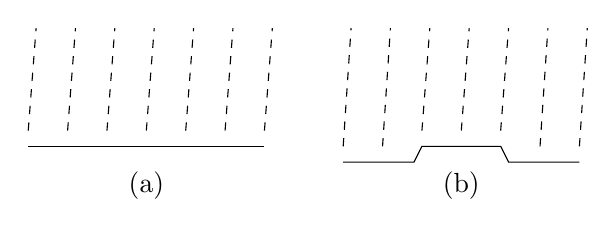
\begin{tikzpicture}[scale=1, transform shape]
      \begin{scope}[shift={(0,0)}]
        \draw (0,0) -- (1,0) -- (2,0) -- (3,0);
        \draw[dashed] (0,0.2) -- (0.1,1.5);
        \draw[dashed] (0.5,0.2) -- (0.6,1.5);
        \draw[dashed] (1,0.2) -- (1.1,1.5);
        \draw[dashed] (1.5,0.2) -- (1.6,1.5);
        \draw[dashed] (2,0.2) -- (2.1,1.5);
        \draw[dashed] (2.5,0.2) -- (2.6,1.5);
        \draw[dashed] (3,0.2) -- (3.1,1.5);
        \node (a) at (1.5, -0.5) {(a)};
      \end{scope}

      \begin{scope}[shift={(4,0)}]
        \draw (0,-0.2) -- (0.9,-0.2) -- (1,0) -- (2,0) -- (2.1,-0.2) -- (3,-0.2);
        \draw[dashed] (0,0) -- (0.1,1.5);
        \draw[dashed] (0.5,0) -- (0.6,1.5);
        \draw[dashed] (1,0.2) -- (1.1,1.5);
        \draw[dashed] (1.5,0.2) -- (1.6,1.5);
        \draw[dashed] (2,0.2) -- (2.1,1.5);
        \draw[dashed] (2.5,0) -- (2.6,1.5);
        \draw[dashed] (3,0) -- (3.1,1.5);
        \node (b) at (1.5, -0.5) {(b)};
      \end{scope}
    \end{tikzpicture}
  \end{center}
  \caption{Demonstrating the process of solar radiation wearing through the
    marble surface, where the center segment is protected by some pigment. Over
  time smooth surfaces of (a) will develop bumps like the surface of (b).}
  \label{fig:raking_light_1}
\end{figure}

This method becomes very useful in determining where different pigments were on
a sculpture and to ascertain the location of the transitions between them.
Since each pigment would protect the underlying medium differently, each
pigment would leave a different sized "bump" on the sculpture. There is little
to gain about the actual color using this method, but it does allow for knowing
where the different colors start and end.

By shining a light almost perpendicular to the surface of the sculpture it is
possible to see these microscopic ridges on the surface. This process is
clearly depicted in figure \ref{fig:raking_light_2}. It can be seen that the
parts of the sculpture that face the light source will be emphasized, and the
parts of the sculpture that face away from the source will be obscured in
shadow. This allows the distinction between different surfaces that may be
impossible to visually see without the enhancement resulting from the shadows
and highlights.

\begin{figure}[htpb]
  \begin{center}
    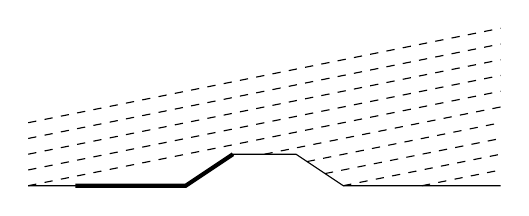
\begin{tikzpicture}[scale=2, transform shape]
      \draw (0,0) -- (1,0) -- (1.3,0.2) -- (1.7,0.2)--(2,0)--(3,0);
      \draw[line width=1.5pt] (0.3,0) -- (1,0) -- (1.3,0.2);
      \draw[dashed] (0.0,0.4) -- (3.0,1.0);
      \draw[dashed] (0.0,0.3) -- (3.0,0.9);
      \draw[dashed] (0.0,0.2) -- (3.0,0.8);
      \draw[dashed] (0.0,0.1) -- (3.0,0.7);
      \draw[dashed] (0.0,0) -- (3.0,0.6);
      \draw[dashed] (1.5,0.2) -- (3.0,0.5);
      \draw[dashed] (1.769,0.153) -- (3.0,0.4);
      \draw[dashed] (1.884,0.077) -- (3.0,0.3);
      \draw[dashed] (2.0,0) -- (3.0,0.2);
      \draw[dashed] (2.5,0) -- (3.0,0.1);
    \end{tikzpicture}
  \end{center}
  \caption{Demonstrating how using raking light will cast shadows caused by
  small ridges on the surface of a material. This allows for the determination
  of where pigments would have been present.}
  \label{fig:raking_light_2}
\end{figure}

This method of raking light does not provide researchers will too much
information about what pigments were actually present on a sculpture, but it
does help in the determination of the regions of different pigments. Thus if a
pigment is determined to be anywhere in the region, it is reasonable to believe
that that pigment was used for the entirety of the region. Using raking light
can be seen in this image of a wall shown in figure
\ref{fig:raking_light_3}\autocite{RLI}.

\begin{figure}[htpb]
  \centering
  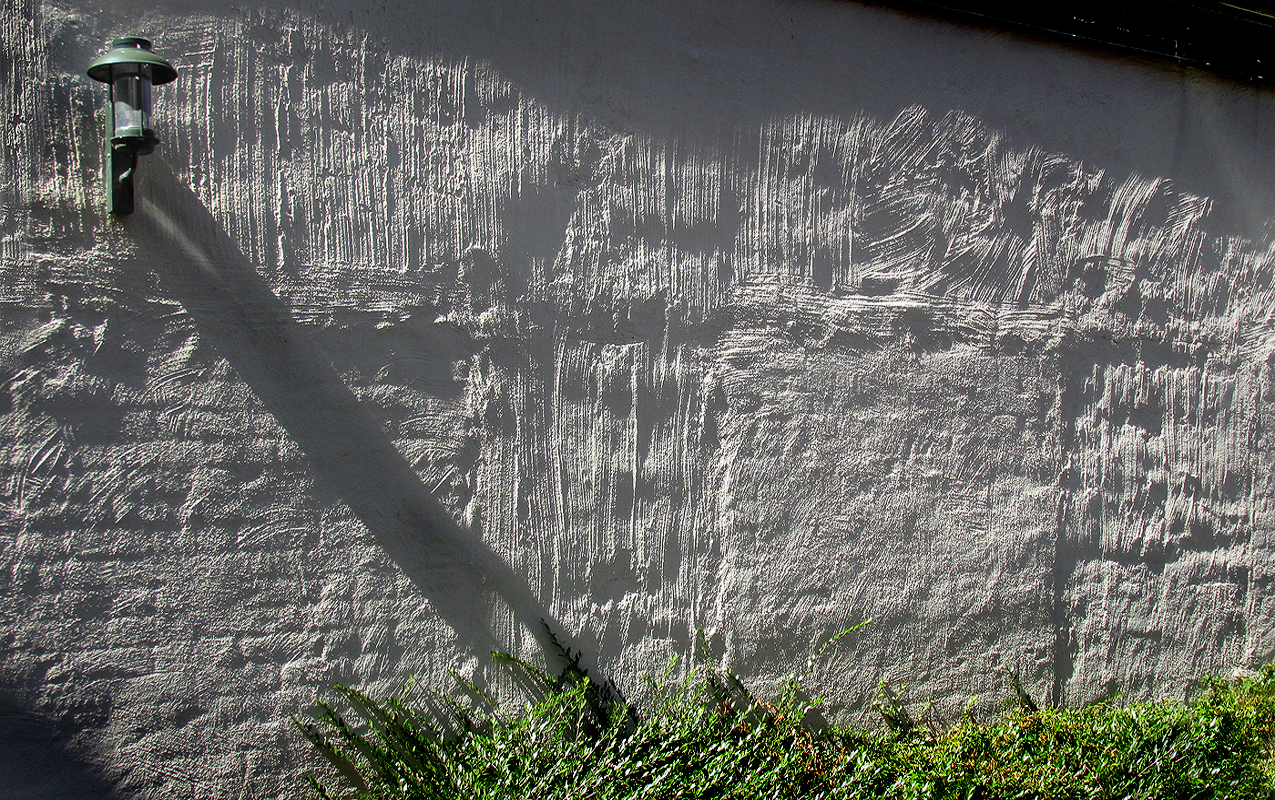
\includegraphics[width=0.5\linewidth]{raking_light.jpg}
  \caption{Raking light on a wall, emphasizing the brush strokes in the
  painting process. This can be used in a similar manner on ancient sculpture.}
  \label{fig:raking_light_3}
\end{figure}

\textbf{UV Florescence} This method begins utilizing the chemical composition
of the pigments themselves in order to assist in determining the colors.
Certain pigments will absorb light in the ultraviolet frequencies and will
remit the light at a lower frequency in the visual spectrum. This method
involves simply shining ultraviolet light on the sculpture, then watching for
any parts of the sculpture that glow when the light is removed. What color the
pigments glow also assists in determining what the original pigment could be.
Using the observations of this method does not necessarily provide a direct
answer to what pigment or colors were used, it certainly assists in narrowing
down the options.

This method is also closely related to the more scientific method of UV vis.
They both use properties of how the pigments interact with ultraviolet light.
Since different pigments interact with ultraviolet light in different ways,
they will also interact differently for different frequencies of ultraviolet
light.

\textbf{UV Visible Spectroscopy} This is the final method that we will explain
in detail. The basis of this process is to use how light interacts with other
objects in the natural world, and how the colors of those objects are then
perceived.

Light from the sun, or from light bulbs, will frequently be white, or off
white. This means that all visible wavelengths of electromagnetic radiation are
present in the light. Every material has specific wavelengths of light which it
will absorb. The light that we observe is the wavelengths of light that a
material does not absorb. For example, consider plants. Plants are green
because they absorb all other wavelengths of visible light, and they reflect
the green light. The wavelengths of light that a material absorbs is called the
absorption spectrum.

There are wavelengths of light that are outside of what is visible to humans.
These wavelengths include ultraviolet rays. The absorption spectrum is not
restricted to the wavelengths of visible light, materials can absorb any
wavelengths of light. This can be seen in sunscreen. Sunscreen in completely
transparent to visible light, but is completely opaque to ultraviolet rays.
This is how it protects one's skin from harmful light.

Every specific chemical possesses a unique absorption spectrum. Experimentally
determining the absorption spectrum of an unknown material, and comparing to
the set of known spectra, it is possible to determine what the unknown sample
consists of, just by looking for matching absorption plots.

Because of this, it is possible to look at the absorption spectrum in the
ultraviolet wavelengths of samples of unknown pigments. Since the visual
absorption spectrum has been damaged by sunlight, it is important to only
consider the UV wavelengths. With the determined spectrum, it is then possible
to compare it to a database of known pigments and narrow the possibilities of
what the sample pigment could be.

There are two methods of how UV-Vis Spectroscopy is implemented. There are the
reflective spectrum and the absorption spectrum methods. For the absorption
method, the material must be placed into a solution or a gas. For the purpose
of analyzing ancient sculpture, this is not often feasible without incurring
some damage to the sculpture by taking a sample.

For the reflective method, it is possible to not alter the original object in
any way. This is perfect for our purposes. This method is done by shining a
beam of light from a tungsten bulb onto the surface of the material. The
material will absorb or reflect specific wavelengths of light, which is
determined by the chemical structure of the pigment. The reason for using a
tungsten light is it produces the most uniform spectrum of light. Most light
sources only produce some wavelengths and not all of them. By using a tungsten
light source, most of the necessary wavelengths of light will be present for
the incident rays.

Once the light has been reflected, it is passed through a diffusing device,
which uses a prism to separate the different wavelengths of light. Then sensors
detect how much of each wavelength was present in the reflected light rays.
Using the ultraviolet wavelengths of light allows one to determine the
structure of the chemical composition of the pigments, and then by comparison
to a known database, it is possible to determine the pigment that was used.

\textbf{Conclusion} All of the methods mentioned here are extremely useful for
the determination of the polychromy of ancient sculpture. However, there is no
single method that can do it alone. Each of these methods are used in
conjunction to assist in furthering researchers' knowledge of a specific
sculpture. Even with all of these methods and many more which were not
mentioned, it is not always possible to ascertain the pigments or even the
colors that were used. However, it is clear that these scientific methods play
a key role in expanding our understanding of these ancient cultures and their
depictions in ancient sculptures. It is important to have an understanding of
the scientific research, in addition to an understanding of the historical
reference frame.  Only with these used together is it possible for one to gain
more insight into the culture of these ancient civilizations. There is no one
single method that can provide all the answers, instead one must use bits and
pieces of information from a diverse collection of sources. Some of these
sources are scientific, some are literary, some are artistic. The importance is
that they are all considered in the overall historical analysis of a piece.

\nocite{*}
\printbibliography

\end{document}
